\chapter[Topic: Immunization]{Topic: Immunization (10\%-15\%)}

\subsection{Information}

\begin{distributions}[Objective]
The Candidate will understand key concepts concerning cash flow matching and immunization, and how to perform related calculations.
\end{distributions}

\begin{outcomes}[Learning outcomes]
The candidate will be able to:
\begin{enumerate}[label = \alph*)]
	\item	Define and recognize the \textit{definitions} of the following terms:
		\begin{itemize}[leftmargin = *]
		\item	Cash flow matching;
		\item	Immunization (including full immunization);
		\item	Redington immunization.
		\end{itemize}
	\item	Construct an investment portfolio to:
		\begin{itemize}[leftmargin = *]
		\item	Redington immunize a set of liability cash flows;
		\item	Fully immunize a set of liability cash flows;
		\item	Exactly match a set of liability cash flows.
		\end{itemize}
\end{enumerate}
\end{outcomes}

\begin{ASM_chapter}[Related lessons ASM]
Section 10: Duration, Convexity, and Immunization
\begin{itemize}[leftmargin = *]
	\item	\nameref{L.-10h}
	\item	\nameref{L.-10i}
	\item	\nameref{L.-10j}
	\item	\nameref{L.-10k}
\end{itemize}
\end{ASM_chapter}

\subsection{Chapter summaries}

\begin{CHPT_SUMM_AUTO}[label = {L.-10h}]{10h. Redington Immunization}
Unless asset cash inflows and liability cash outflows are \textbf{exactly} matched, changes in interest rates (up or down) can cause us to be unable to pay the liabilities.
\begin{description}
	\item[Immunization]	Protecting a financial enterprise from changes in interest rates.
\end{description}


Redington defined \textbf{Redington Immunization} with 3 principles to protect a company against \textbf{small} changes in interest rates:
\begin{enumerate}
	\item	PV assets = PV liabilities
	\item	Duration assets = Duration liabilities
	\item	Convexity assets > Convexity liabilities
\end{enumerate}

Conditions 2 and 3 ensure a small change in the interest rate on either side of $i_{0}$ will result in a net increase of the PV of the assets over the PV of the liabilities.

Equivalently, we can write these as:
\begin{enumerate}
	\item	$P_{A} = P_{L}$
	\item	$P'_{A} = P'_{L}$
	\item	$P''_{A} = P''_{L}$
\end{enumerate}

If we define the NPV $P = P_{A} - P_{L}$ we can write them as:
\begin{enumerate}
	\item	$P = 0$
	\item	$P' = 0$
	\item	$P'' > 0$
\end{enumerate}

Note that conditions 2 and 3 are the conditions for a relative minimum at $i = i_{0}$ thereby ensuring that the NPV is concave upwards at $i_{0}$.
\end{CHPT_SUMM_AUTO}

\begin{CHPT_SUMM_AUTO}[label = {L.-10i}]{10i. Full Immunization}
Full immunization protects a company against \textbf{any} change in the interest rate, no matter the size. Essentially, we ensure that there are 2 asset cash inflows: one before the liability cash outflow and one after.

Conditions are:
\begin{enumerate}
	\item	PV assets = PV liabilities
	\item	Duration assets = Duration liabilities
	\item	There is one asset cash inflow before the liability cash outflow and one after it.
\end{enumerate}
\end{CHPT_SUMM_AUTO}

\begin{CHPT_SUMM_AUTO}[label = {L.-10j}]{10j. A Note on Rebalancing}
In the real world, assets and liabilities change regularly and a company must \textbf{rebalance} its portfolio often. Another possible reason why company may no longer be immunized is that duration changes as time goes by.
\end{CHPT_SUMM_AUTO}

\begin{CHPT_SUMM_AUTO}[label = {L.-10k}]{10k. Immunization by Exact Matching ("Dedication")}
Exact matching ensures that the asset cash flow at each time $t$ is equal to the corresponding liability cash outflow at that time, i.e., $A_{t} = L_{t}, \forall t$.

\begin{itemize}[leftmargin = *]
	\item	This means that changes in interest rates wouldn't have any incidence as all cash flows are exactly matched.
	\item	This is also known as \textbf{dedication}, cash flow matching, exact matching and asset-liability matching.
\end{itemize}

There are a few problems:

\begin{itemize}[leftmargin = *]
	\item	Cash inflows are not always predictable (bonds may be called, mortgages prepaid, etc.).
	\item	Cash outflows are often only estimates (may depend on probabilities of death, sickness, etc., or customer actions like withdrawals).
	\item	Assets may not be available to exactly match liabilities.
	\item	This rigid method may not lead to the best yield rate.
\end{itemize}

To solve these problems, we must start from the end and work ourselves backward to the beginning. The book has an example and this is the end result:
\begin{center}
	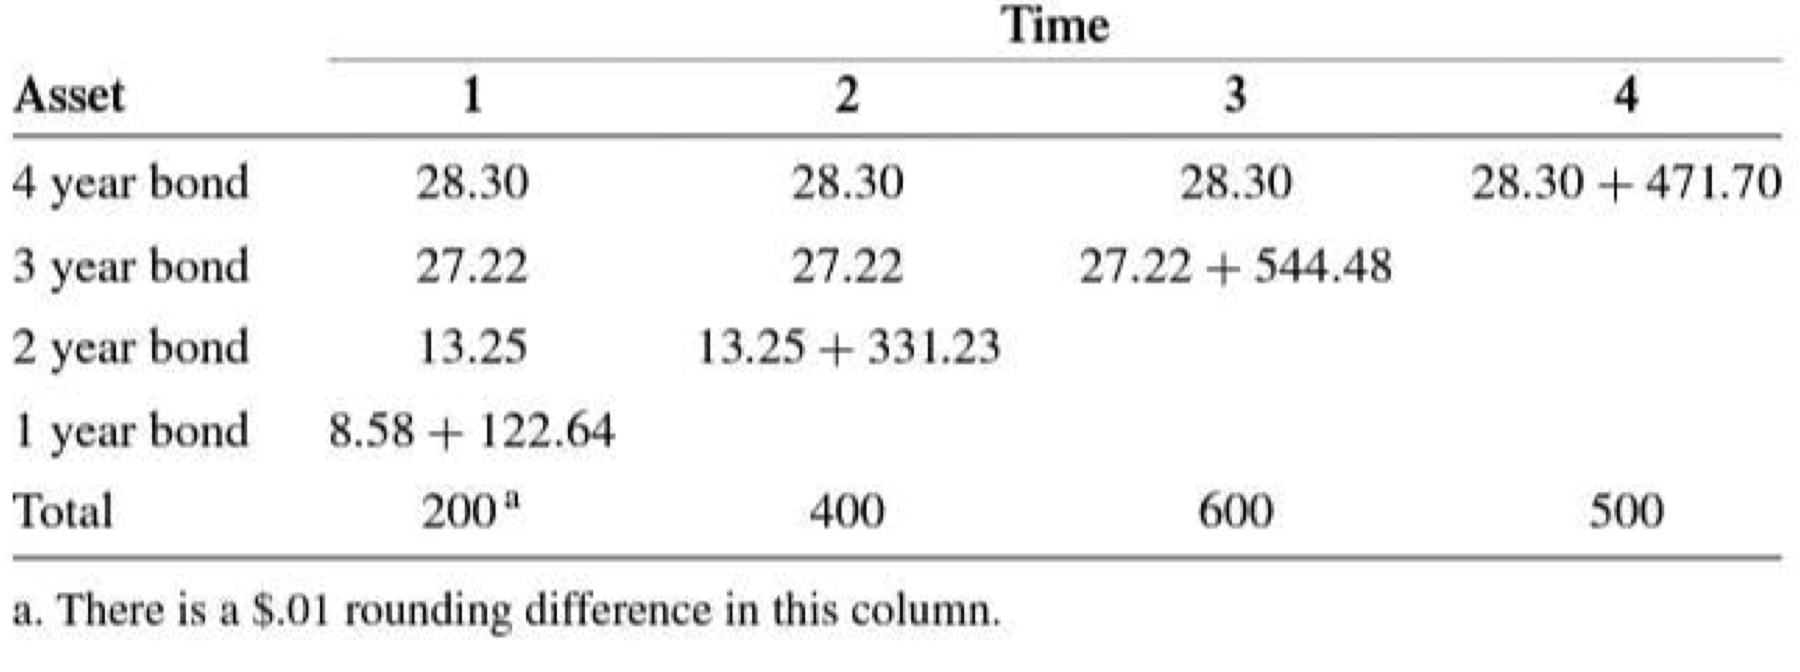
\includegraphics[scale=0.4]{img/immunization-exact.png}
\end{center}
\end{CHPT_SUMM_AUTO}



\begin{YTB_vids}[Vidéos YouTube]
\begin{itemize}
	\item	\href{https://www.youtube.com/watch?v=F7XnR7sKWiE&list=PL_KGEFWqEaTBbYDupRektHIMG0G9u-Ru-&index=54&t=0s}{Macaulay Duration}.
	\item	\href{https://www.youtube.com/watch?v=rdDfmlerTcI&list=PL_KGEFWqEaTBbYDupRektHIMG0G9u-Ru-&index=53&t=0s}{Modified Duration}.
\end{itemize}
\end{YTB_vids}

\begin{itemize}
	\item	MacD = the weighted-average \textbf{maturity} of the CF from a bond.
	\item	ModD = sensitivity of a bond's price to yield.
\end{itemize}